!en \section{Stable Decisions}
!de \section{Stabile Entscheidungen}



!en X

!de In diesem Beispiel sollten wir etwas sinnvolleres unternehmen. Das werden wir unter Beibehaltung des Programmrahmens. Es bleibt also zunächst bei einem Programm der 'zweiten Form': Ein Programm, dass etwas in seiner Endlossschleife tut.



!en X

!de Das Programm speichert einen von zwei Zuständen ;-) und stellte das Licht an oder aus, abhängig vom gespeicherten Zustand. Diese Erklärung ist nicht ganz richtig. Darum versuche ich es noch einmal.



!en X

!de Das Programm erkennt ein Signal am Eingang, an einem Phasenwechsel. Ein vollständiges Signal besteht aus dem Wechsel des Eingangspegels von HOCH nach NIEDRIG und wieder nach HOCH. Das Programm interessiert sich nur für den Wechsel, worauf auch wir uns immer konzentrieren sollten. Wenn der Signalpegel von HOCH nach NIEDRIG wechselt, kehrt unser Programm den Status der LED um. Wenn das Licht AN war, geht es AUS und umgekehrt. 



!en X

!de Das Ausgangssignal wird umgekehrt wenn der Eingangspegel von HOCH nach NIEDRIG wechselt weil durch die Verwendung eines 'pull up' Widerstandes der Pegel am Eingang HOCH ist, während der Knopf \textit{nicht} gedrückt wird. Auf den Wechsel von HOCH nach NIEDRIG zu reagieren bedeutet also, die Aktion in dem Moment auszulösen wenn der Schalter gedrückt wird.



!en X

!de Wir dürfen davon ausgehen, dass das das ist, was der Benutzer des Programms höchstwahrscheinlich erwartet. Denn ein solches Verhalten entspricht den meisten Lichtschaltern mit denen wir konfrontiert werden.



!en X

!de Das \textit{elektrische} Signal, auf das unser MC am gewählten Eingangsbein wartet ist der Wechsel des Spannungszustandes von HOCH (VCC) nach NIEDRIG (GND). Um exakt zu sein sollten wir die Erwartungshaltung so formulieren:

\begin{center}
!en The \emph{Signal} the MC is waiting for is the \emph{Change} form VCC to GND.
!de Das \emph{Signal} auf dass der MC wartet ist der \emph{Wechsel} von VCC nach GND.
\end{center}



!en X

!de Zum ersten Mal (und hoffentlich nicht zu oft) haben wir uns mit einem dynamischen Zustand zu beschäftigen. Wenn der Wechsel des Pegels das Signal ist, müssen wir den Umstand 'hat gewechselt' erkennen. Wenn also der Pegel NIEDRIG erkannt wird, \textit{unmittelbar} nachdem der Pegel HOCH war (also in der nahen Vergangenheit!), haben wir es gewissermassen mit Vergangenheitsbewältigung zu tun. Dafür muss sich unser Programm zum ersten Mal in einem Verarbeitungszyklus an einen vergangenen Pegel/Messwert aus dem vorherigen Verarbeitungszyklus erinnern.


!en X:

!de Und das geht so:

\begin{lstlisting}
; LED/S004_stable-decisions.asm

.DEVICE atmega8

.org 0x0000
            rjmp    start

start:
            sbi     DDRB,         5
            cbi     DDRB,         0
            sbi     PORTB,        0

            ldi     r16,          1

main:
            sbic    PINB,         0
            rjmp    led_keep
            tst     r16
            breq    led_ok
            clr     r16
            sbis    PINB,         5
            rjmp    led_on
            cbi     PORTB,        5
            rjmp    led_ok
led_on:
            sbi     PORTB,        5
            rjmp    led_ok
led_keep:
            ldi     r16,          1
led_ok:
            rjmp    main
\end{lstlisting}



!en X:

!de Wie man leicht erkennen kann, ist dieser Programmcode nicht leicht zu verstehen. Um dieses Missstand abzustellen, wollen wir ein paar symbolische Namen in die Suppe rühren. Die Grundlagen sind:

\begin{itemize}
!en   \item \texttt{.equ} means: 'a name for a value'
!de   \item \texttt{.equ} heisst: 'ein Name für einen Wert' (Zahl oder Text)
!en   \item \texttt{.def} means: 'a name for an entity'
!de   \item \texttt{.def} heisst: 'ein Name für ein Ding' (z.B: CPU Register)
\end{itemize}



!en X

!de \texttt{DDRB} zum Beispiel ist bereits eine Nummer. Diese Nummer ist in einer Datei hinterlegt, die durch die Geräteauswahl bestimmt und geladen wird. In unserem Fall soll \texttt{DDRB}, unabhängig von seinem Wert, unsere Eingangs- und Ausgangsbeine bezeichnen. Wir bilden den Namen aus \texttt{ctl} als Präfix für 'Control Port' und \texttt{IO} als Abkürzung für Input\&Output. Das ergibt \texttt{ctlIO}.



!en X

!de Ein anderes Beispiel: \texttt{bit} für 'Bitnummer' und \texttt{Input} für Inputbit, macht \texttt{bitInput}. Oder \texttt{b} für 'Byte' und \texttt{Status} für 'Statusregister' macht \texttt{bStatus}



!en X

!de Es spricht nichts dagegen, eine eigene Namenskonvention zu entwickeln, eine sinnvolle Struktur sollte sich daraus aber ergeben. So könnte man beispielsweise auch \texttt{InputCtl} verwenden und \texttt{InputBit} usw. Wie es einem am leichtesten Fällt oder wie es einem vorgeschrieben wird.

\begin{lstlisting}
; LED/S005_stable-decisions+symbols.asm

.DEVICE atmega8

.equ ctlIO     = DDRB    ; DDRB  is our I/O control register
.equ prtIO     = PORTB   ; PORTB is our I/O output port register
.equ pinIO     = PINB    ; PINB  is our I/O input pin register

.equ bitOutput = 5       ; bit 5 is our output bit
.equ bitInput  = 0       ; bit 0 is our input bit

.equ FALSE     = 0       ; 0 will be FALSE or OFF
.equ TRUE      = 1       ; 1 will be TRUE  or ON

.def bStatus   = r16     ; the last state will be stored in 'r16'
\end{lstlisting}



!en X

!de Diese Massnahme macht den Code meistens leichter lesbar und somit leichter zu verstehen und zu interpretieren. Jener sieht dann so aus (fast schon wie eine Hochsprache):

\begin{lstlisting}
.org 0x0000
            rjmp    start

start:
            sbi     ctlIO,        bitOutput
            cbi     ctlIO,        bitInput
            sbi     prtIO,        bitInput

            ldi     bStatus,      HIGH

main:
            sbic    pinIO,        bitInput
            rjmp    led_keep
            tst     bStatus
            breq    led_ok
            clr     bStatus
            sbis    pinIO,        bitOutput
            rjmp    led_on
            cbi     prtIO,        bitOutput
            rjmp    led_ok
led_on:
            sbi     prtIO,        bitOutput
            rjmp    led_ok
led_keep:
            ldi     bStatus,      HIGH
led_ok:
            rjmp    main
\end{lstlisting}


!en X

!de Zusätzlich vereinfacht die Verwendung von Symbolen Änderungen. Kürzlich mussten wir \texttt{bitInput} von \texttt{4} auf \texttt{0} ändern. Durch die Verwendung symbolischer Namen war diese Änderung leichter und mich weniger Risiko zu machen als bei der Verwendung unmittelbarer Werte. Man kann nicht einfach alle \texttt{4}en im Text durch \texttt{0}en ersetzen, darf bei einer solchen Änderung aber auch keine der zu ändernden \texttt{4}en vergessen. Mit symbolischen Namen allerdings muss man den Programmtext nur an einer einzigen Stelle ändern.



!en X

!de Doch auch wenn sich der Text mit Symbolen angenehmer lesen lässt, ist er, was man nicht auf den ersten Blick erkennen kann, noch nicht ohne weiteres zu verstehen. Darum zeigen wir hier für das erste Mal einen Programmablaufplan. Aus gutem Grund verwenden wir gleich zwei davon. Wir brauchen zwei um einen wesentlichen Punkt der Assemblerprogrammierung zu zeigen.



!en X

!de Wir müssen nicht nur verfolgen \textit{was} wir tun müssen, sondern auch \textit{wie} das getan wird.



!en \subsection{WHAT to do}
!de \subsection{\textit{Was} getan wird}

\begin{enumerate}
!en   \item Initialise system and devices
!de   \item Das System und die Geräte initialisieren
!en   \item Read input
!de   \item Eingang auslesen
!en   \item Check for 'input bit was HIGH and became LOW'
!de   \item Prüfen ob 'Eingang war HIGH und ist jetzt LOW' vorliegt
!en   \item If so: invert LED status
!de   \item Wenn ja: Umkehren des LED Status
!en   \item Restart at (2)
!de   \item Neu starten bei (2)
\end{enumerate}



!en \subsection{HOW to do it}
!de \subsection{\textit{Wie} es getan wird}



!en X

!de Um einen Eindruck zu erhalten wie es getan wird, werfen wir einen Blick auf den Ablaufplan.

\begin{figure}[htbp]
  \centering
  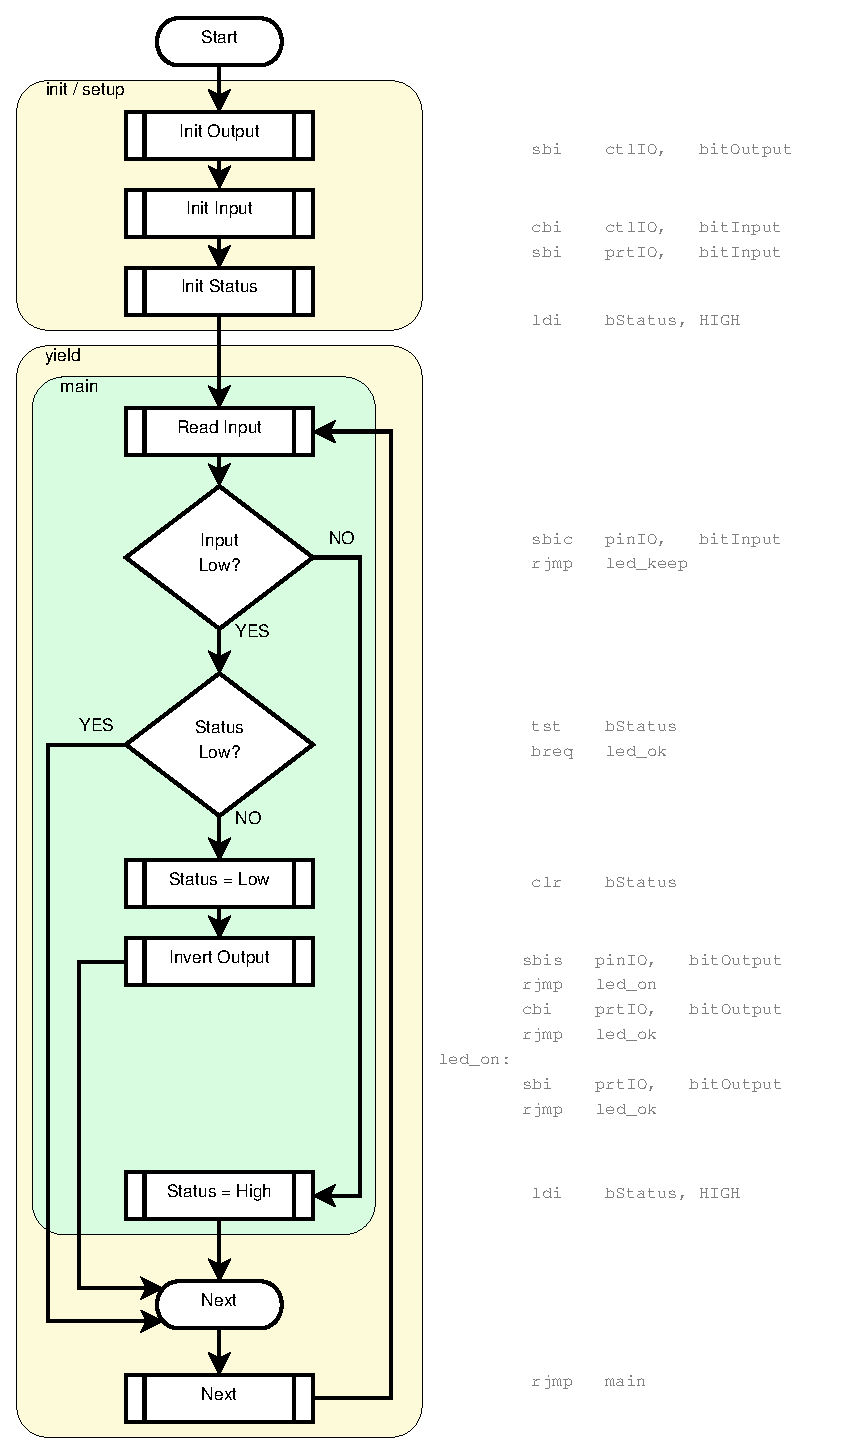
\includegraphics[height=0.95\textheight]{LED/S005_stable-decisions+symbols.eps}
!en   \caption{Stable Decisions - Flow Diagram}
!de   \caption{Stabile Entscheidungen - Ablaufplan}
  \label{S005FlowDiagam}
\end{figure}



!en X

!de Der grösster Störfaktor in der Informatik ist bekanntlich der Anwender. Nicht nur, dass seine Erwartungen von den Konzepten der Entwickler abweichen, es beginnt schon damit, dass er, in seinem Aufbau als Bioeinheit, unvorstellbar langsam ist. Die unglaubliche Langsamkeit des Anwenders ist ein technisches Problem, die Erwartungshaltung an die Art wie Geräte funktionieren ein ökonomisches. Wenn der gemeine Anwender unser Gerät nicht akzeptiert, wird er es nicht kaufen und wir haben nichts zu essen.



!en \subsubsection{Slow users}
!de \subsubsection{Die unglaubliche Langsamkeit des Anwenders}



!en X

!de Eine Bioeinheit drückt einen Knopf und unser Gerät hat zu reagieren. Dummer Weise prüft unser Gerät den Schalter vielleicht 1.000.000 Mal in jeder Sekunde. Ein Mensch z.B. mag einen Knopf sehr schnell drücken und den Kontakt im Schalter für 0.2s schliessen. Unser Gerät erkennt während dessen 200.000 Mal, dass der Schalter durchgeschaltet ist. Dies wohlgemerkt bei einem ganz schnellen Menschen. Was der Mensch aber erwartet ist:

\begin{center}\textit{
!en Change the light ones as I press (in my view) the button ones!
!de Schalte das Licht einmal um wenn ich (aus meiner Sicht) den Knopf einmal drücke. 
\end{center}}



!en X

!de Das Gerät darf also nur einmal umschalten auch wenn es 200.000 Mal feststellt, dass der Knopf gedrückt ist. Aus diesem Grund halten wir uns am Wechsel des Schaltzustandes fest um den Vorgang des Schaltens zu erkennen. Wir müssen also erkennen, ob sich der Zustand am Eingangbein unseres Microcontrollers \textit{geändert} hat! Dazu benötigen wir einen Zwischenspeicher, der den Schaltzustand bei der vorherigen Messung speichert. Wechselt dieser Zustand, müssen wir das Licht umschalten.



!en \subsubsection{Flickering}
!de \subsubsection{Prellen}



!en X

!de Problematisch dabei ist, dass elektrische Schalter prellen. Das heisst, sie stellen den Kontakt nicht so her wie wir es annehmen. Anstatt einmal einzuschalten, prallen die mechanischen Elemente des Schalters beim Aufprall voneinander ab und trennen die Verbindung wieder, um sie Millisekunden später dank der Elastizität der Schaltelemente wieder zu schliessen. Das kann sich unterschiedlich oft wiederholen. Wie das genau abläuft ist von unzähligen Faktoren abhängig. Die elektrische Konsequenz ist vereinfacht in Grafik \ref{S005SignalDiagam-Flicker} dargestellt.



!en X

!de Diesem Problem begegnen wir elektronisch. Anstatt mit dem Schalter einfach direkt das Bein des Eingangs am Schaltkreis auf Masse zu ziehen, verzögern wir die Spannungsänderung mit einem Kondensator wie in Abbildung \ref{S005FlickerReduction}.


%\begin{wrapfigure}{R}{0.25\textwidth}
\begin{figure}[htbp]
  \centering
%  \begin{center}
    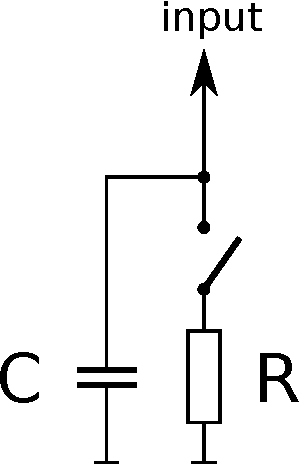
\includegraphics[width=0.24\textwidth]{LED/S005_stable-decisions_no-flicker.pdf}
%  \end{center}
!en   \caption{Flicker reduction}
!de   \caption{Prellunterdrückung}
  \label{S005FlickerReduction}
\end{figure}




!en X

!de Die Auswirkung dieser Massnahmen wird in Abbildung \ref{S005SignalDiagam} dargestellt. Grafik \ref{S005SignalDiagam-Ideal} zeigt den Spannungsverlauf am Eingangsbein des Microcontrollers wie wir ihn uns wünschen. In der Grafik \ref{S005SignalDiagam-Ideal+C} kann man erkennen, wie sich das Hinzufügen eines Kondensators (und des Widerstandes) darauf auswirken würde. Beim idealen rechteckigen Spannungsverlauf, wäre der Umschaltzeitpunkt identisch mit dem Zeitpunkt des Signalwechsels am Eingang des Microcontrollers. Durch den Kondensator wird dieser Umschaltzeitpunkt verzögert.




!en X

!de Den vereinfachten tatsächlichen Spannungsverlauf beim Schalten des Schalters zeigt Grafik \ref{S005SignalDiagam-Flicker} während Grafik \ref{S005SignalDiagam-Flicker+C} demonstriert, auf welche Weise uns der Einsatz eines Kondensators, der über einen Widerstand geladen wird, vor unkontrollierten Signalen schützt.




!en X

!de Die Kreise '\texttt{a}' und '\texttt{b}' umkreisen die Punkte an denen der tatsächliche Spannungsverlauf die Umschaltschwellen von \texttt{1} nach \texttt{0} (bzw. umgekehrt) schneidet und am Microcontoller tatsächlich der Eingangspegel wechselt. Die vertikale rote Linie in den Grafiken \ref{S005SignalDiagam-Ideal+C} und \ref{S005SignalDiagam-Flicker+C} zeigen den Moment, ab dem unser Programm den Wechsel der Eingangsspannung feststellen kann.



\begin{figure}%[htbp]
  \begin{subfigure}[htbp]{0.485\textwidth}
    \centering
    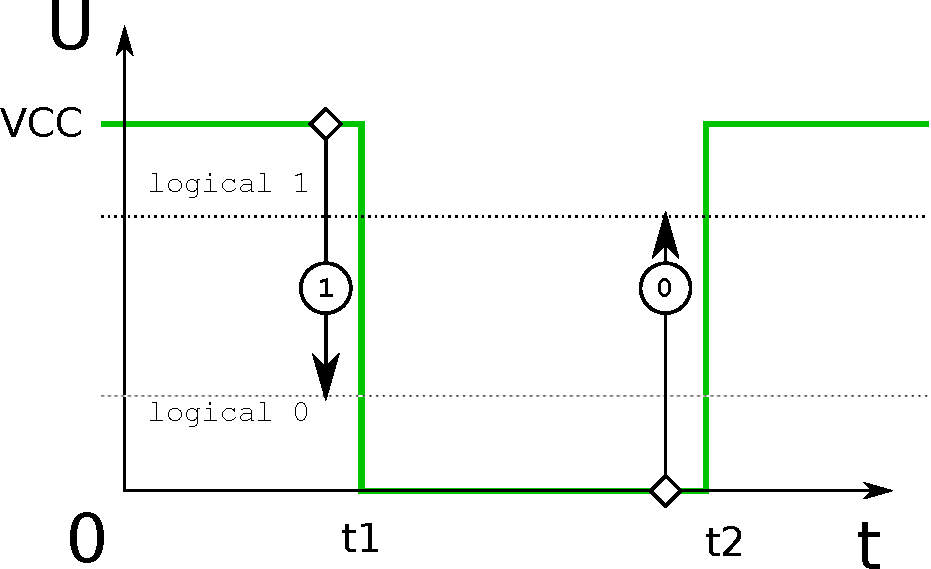
\includegraphics[width=\textwidth]{LED/S005_stable-decisions_ideal_signal.pdf}
    \caption{ideal}
    \label{S005SignalDiagam-Ideal}
  \end{subfigure}
  \quad
  \begin{subfigure}[htbp]{0.485\textwidth}
    \centering
    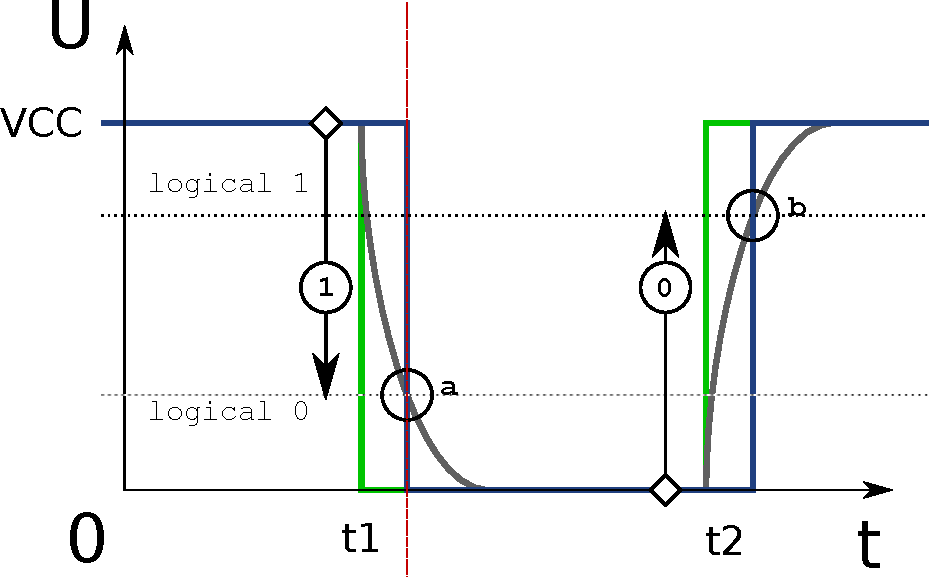
\includegraphics[width=\textwidth]{LED/S005_stable-decisions_ideal_signal+C.pdf}
!en     \caption{ideal + Capacitor}
!de     \caption{ideal + Kondensator}
    \label{S005SignalDiagam-Ideal+C}
  \end{subfigure}

  \begin{subfigure}[htbp]{0.485\textwidth}
    \centering
    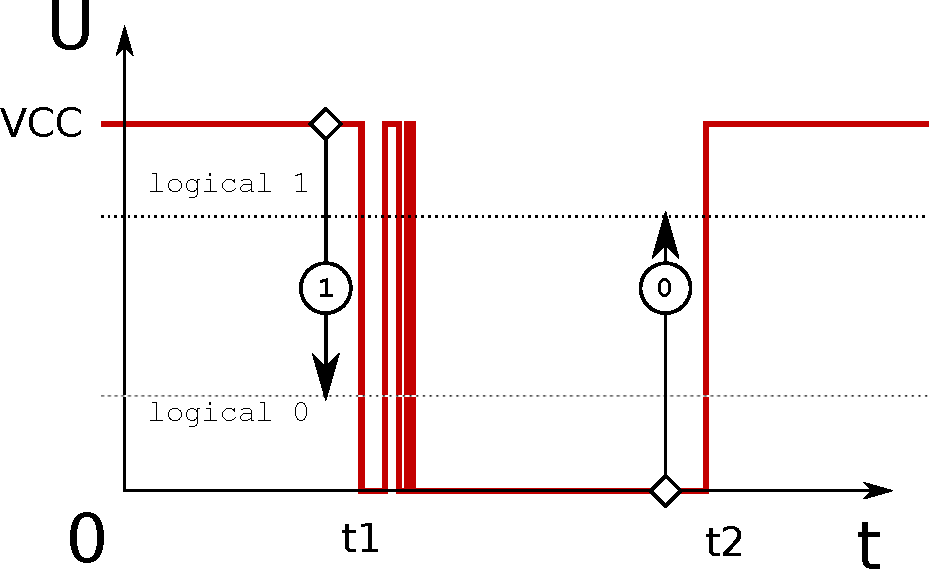
\includegraphics[width=\textwidth]{LED/S005_stable-decisions_ideal_signal+flicker.pdf}
!en     \caption{flickering}
!de     \caption{prellend}
    \label{S005SignalDiagam-Flicker}
  \end{subfigure}
  \quad
  \begin{subfigure}[htbp]{0.485\textwidth}
    \centering
    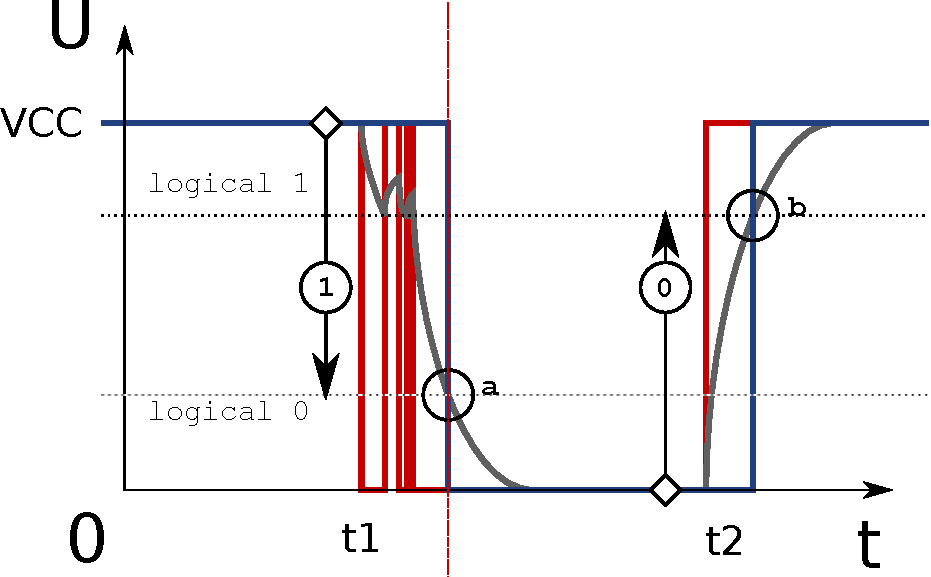
\includegraphics[width=\textwidth]{LED/S005_stable-decisions_ideal_signal+flicker+C.pdf}
!en     \caption{flickering + Capacitor}
!de     \caption{prellend + Kondensator}
    \label{S005SignalDiagam-Flicker+C}
  \end{subfigure}
!en   \caption{Stable Decisions - Signal Diagram}
!de   \caption{Stabile Entscheidungen - Signaldiagramme}
  \label{S005SignalDiagam}
\end{figure}

%\begin{figure}[htbp]
%  \centering
%  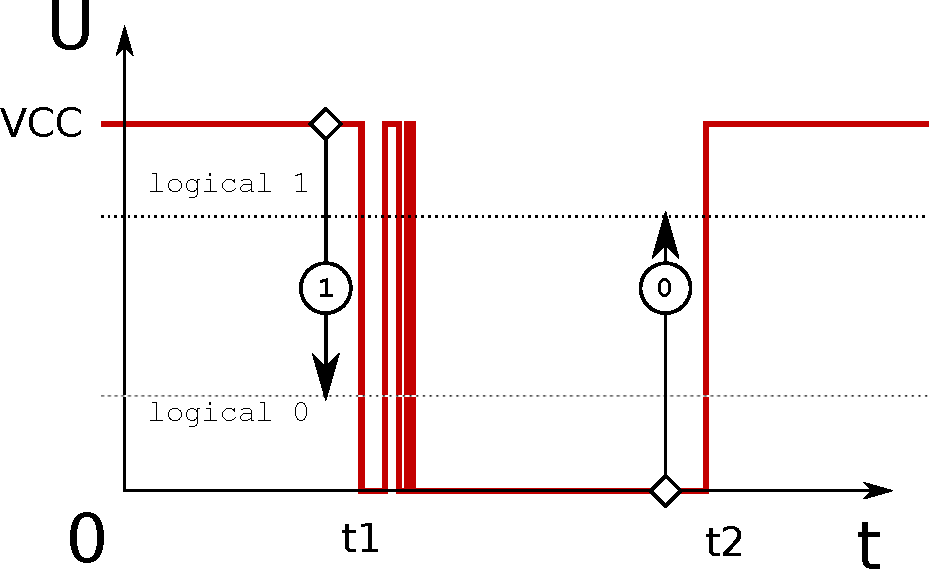
\includegraphics[width=80mm]{LED/S005_stable-decisions_ideal_signal+flicker.pdf}
%  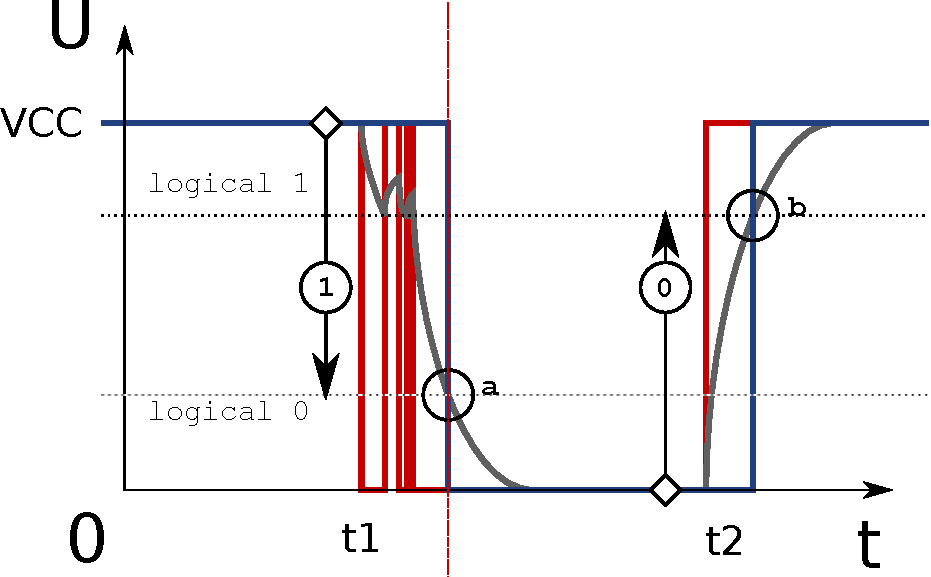
\includegraphics[width=80mm]{LED/S005_stable-decisions_ideal_signal+flicker+C.pdf}
%!en   \caption{Stable Decisions - Signal Diagram flickering without and with Capacitor}
%!de   \caption{Stabile Entscheidungen - Signaldiagramm prellend ohne und mit Kondensator}
%  \label{S005SignalDiagam-ideal+flicker+C}
%\end{figure}



!en X

!de Die blaue Linie in Grafik \ref{S005SignalDiagam-Flicker+C} zeigt den Verlauf des Pegels am Eingang nach dem Bedienen des Schalters, dessen Folgen in der roten Linie zu sehen sind. Man könnte den Eindruck gewinnen, als träte infolge der Kondensatorschaltung eine nennenswerte Schaltverzögerung ein. Dies ist aber nicht der Fall. Die Verzögerung liegt, je nach Dimensionierung des Kondensators und des Widerstandes im Bereich von Microsekunden oder Millisekunden. Eine Verzögerung also, die also nur für Maschinen spürbar ist. Die Grafiken in Abbildung \ref{S005SignalDiagam} täuschen über die wahren Verhältnisse hinweg.



!en \subsubsection{Fast feedback}
!de \subsubsection{Schnelle Rückmeldung}



!en X

!de Unser einziges Rückmeldegerät, mit dem wir dem Anwender unserer Applikation auch nur irgend etwas anzeigen können ist die angesteuerte Lampe/LED. Es gibt sonst nichts. Darum bleibt uns als Kommunikationsschnittstelle nur die angesteuerte Lichtquelle selbst. Auch wenn es in manchen Filmen cool erscheinen mag, wenn Akteure ohne Rückmeldungen an komplizierten Anlagen herumspielen und irgendwo in der Welt passiert etwas, die normale Bioeinheit erwartet eine 'sofortige Reaktion' für jede erfolgreiches Aktion. Passiert das nicht, wird es für den Nutzer schwierig.



!en X

!de Wie bereits erwähnt, zwingt uns diese Erwartungshaltung dazu, auf das Auftreten der ersten Schaltflanke im Schaltzyklus (HOCH nach NIEDRIG oder \texttt{1} nach \texttt{0}) zu reagieren. Wir kümmern uns nur um den Moment, in dem der Eingangspegel abfällt. Das ermöglicht uns auf die beiden wichtigen Aufgaben zu reagieren die vor uns stehen.

\begin{itemize}
!en   \item Give feedback as fast as possible
!de   \item So schnell wie möglich Rückmeldung geben
!en   \item Switch only ones if the user switches (in his eyes) ones
!de   \item Nur einmal schalten wenn der Nutzer glaubt, nur einmal geschaltet zu haben
\end{itemize}



!en \subsection{Finding the event}
!de \subsection{Das richtige Ereignis finden}



!en X

!de Für den Microcontroller erscheint alles was Menschen tun und erleben regelrecht endlos langwierig. Einmal ist der Schalter für Millionen Arbeitszyklen gedrückt, dann wieder für Milliarden von Zyklen losgelassen. In all dieser endlosen Langeweile passiert manchmal etwas. Um unseren Moment zu finden, muss unser Programm feststellen, dass sich etwas geändert hat.



!en X

!de Änderungen können nur im Vergleich zwischen zwei Zuständen festgestellt werden! Messen können wir zur gleichen Zeit aber nur einen Zustand. Das heisst, unser Programm muss sich merken, wie der Zustand bei der letzten Messung war um diesen mit der aktuellen Messung zu vergleichen.



!en X

!de War der Zustand eben noch HOCH und wurde in der Aktuellen Messung als NIEDRIG festgestellt ist das lang ersehnte Ereignis eingetreten. Dann muss das Programm handeln, also den Schaltzustand der LED umkehren.



!en \subsection{And some modesty}
!de \subsection{Programmierte Umsicht}


!en X

!de In Rücksichtnahme auf die Dinge, die noch kommen werden, müssen wir Umsicht walten lassen. Die Endlosschleife, die unser Programm am Leben und um Zaum hält, führt (ganz allgemein) einige wichtige Aufgaben aus:

\begin{itemize}
!en   \item It mostly contains the main program
!de   \item Sie enthält den grössten Teil des Hauptprogramms
!en   \item It possibly consist of multiple parts
!de   \item Dieses Programm besteht vielleicht aus mehreren Teilen
!en   \item It consist of an undefined amount of functional separate program parts
!de   \item Wenn es Teile gibt, haben diese völlig verschiedenen Aufgaben
\end{itemize}



!en X

!de Darum müssen wir darauf achten, dass wir keine voreiligen Schlüsse ziehen und Programmteile überspringen, in der Annahme (=scheinbare Gewissheit) dass darin nichts mehr passieren würde.



So we have to ensure, to don't make any shortcut back to the 'main' label. As there can only be one Highlander, there can only be one jump back to 'main'. This jump resides at the very end of the main sequence. Like this:

\begin{lstlisting}
main:

  A_begin:
            block     A or goto to end of block A
  A_end:

  B_begin:
            block     B or goto to end of block B
  B_end:

  C_begin:
            block     C or goto to end of block C
  C_end

mein_end:
            finalise
            rjmp      main
\end{lstlisting}

In our flow diagram one part has to reach the next part regardless of how the program is flowing. The rounded rectangle 'next' represents the central point behind our (currently) one part. This is the position where the next program part would follow in the same manner.

